\chapter{Span}
\section{Spans of Vectors}
Knowing whether two vectors are linearly dependent or independent allows us to 
accurately describe the span of those two vectors (this expands to include any 
number of vectors). In the previous chapter, we saw that linear combinations of 
two linearly dependent vectors can only make vectors that lie on the same line 
as the two starting vectors. We saw this in 2D, but it also applies to 3D 
vectors. Consider the two vectors $\mathbf{u} = \left[ 2, 4, 3 \right]$ and 
$\mathbf{v} = \left[ 4, 8, 6 \right]$, shown in figure \ref{fig:3d_vectors}. 

\begin{figure}[htbp]
\centering
\tdplotsetmaincoords{80}{130} 
\begin{tikzpicture} [scale=4, tdplot_main_coords, axis/.style={->,black}, 
vector/.style={-stealth,blue,very thick}, 
vector guide/.style={dashed,black}]

%standard tikz coordinate definition using x, y, z coords
\coordinate (O) at (0,0,0);

%draw axes
\draw[axis] (0,0,0) -- (1.5,0,0) node[anchor=north east]{$x$};
\draw[axis] (0,0,0) -- (0,0.9,0) node[anchor=north west]{$y$};
\draw[axis] (0,0,0) -- (0,0,0.9) node[anchor=south]{$z$};

%draw a vector from O to P
\draw[vector] (O) -- (0.2, 0.4, 0.3) node[above] {\textbf{u}};
\draw[vector guide] (0.2,0,0) -- (0.2,0.4,0);
\draw[vector guide] (0.0,0.4,0) -- (0.2,0.4,0);
\draw[vector guide] (0.2,0.4,0) -- (0.2,0.4,0.3);

\draw[vector] (O) -- (0.4, 0.8, 0.6) node[above] {\textbf{v}};
\draw[vector guide] (0.4, 0, 0) -- (0.4, 0.8, 0);
\draw[vector guide] (0, 0.8, 0) -- (0.4, 0.8, 0);
\draw[vector guide] (0.4, 0.8, 0) -- (0.4, 0.8, 0.6);
\end{tikzpicture}
\caption{3-dimensional vectors, \textbf{u} and \textbf{v}}
\label{fig:3d_vectors}
\end{figure}
\index{span}
Notice that these two vectors are colinear (that is, they are on the same 
line), therefore they are linearly dependent and any combination of \textbf{u} 
and \textbf{v} will lie on the same line as \textbf{u} and \textbf{v}. 
Therefore, we say the \textit{the span of} \textbf{u} \textit{and} \textit{v} 
\textit{is a line}. In fact, for any size list of linearly dependent vectors 
(whether it's one vector or one hundred), the span of that list is a line. 

Now that you have a sense of what a span is, it is time for the formal 
mathematical definition. A vector span is the collection of vectors obtained 
by scaling and combining the original set of vectors in all possible 
proportions. Formally, if the set $S = \{\mathbf{v_1}, \mathbf{v_2}, \dots, 
\mathbf{v_n}\}$ contains vectors from a vector space $V$, then the span of $S$ 
is given by:

\begin{equation}
\text{Span}(S) = \{a_1 \mathbf{v_1} + a_2 \mathbf{v_2} + \dots + a_n 
\mathbf{v_n} : a_1, a_2, ..., a_n \in \mathbb{R}\}
\end{equation}

This means that any vector in the Span$(S)$ can be written as a linear 
combination of the vectors in $S$.

\subsection{Spans of Independent Vectors}
What if our list of vectors aren't all linearly dependent on each other? We've 
seen in 2 dimensions that any two independent vectors can be linearly combined 
to create any vector in $\mathbb{R}^2$. So, the span is described as a 
\textit{plane} (in fact, it is the entire $xy$-plane, which we also call 
$\mathbb{R}^2$). How does this expand to 3-dimensional vectors? 
\index{plane}
Let's again consider two 3-dimensional vectors: $\mathbf{u} = \left[2, 4, 3 
\right]$ and $\mathbf{v} = \left[ 2, 1, 0 \right]$, as shown in figure 
\ref{fig:3d_ind}.

\begin{figure}[htbp]
\centering
\begin{tikzpicture} 
\begin{axis}[axis lines = center, x={(-0.3cm, -0.3cm)}, y={(.5cm, -0.1cm)}, 
z = {(0cm, 0.5cm)}, xmin = 0, ymin = 0, zmin = 0, xmax = 5, ymax = 5, 
zmax = 5, ticks=none, xlabel = {$x$}, ylabel = {$y$}, zlabel = {$z$}]
    \draw[blue, thick, -latex] (0,0,0) -- (2, 4, 3) node[above] {\textbf{u}};
    \draw[blue, thick, -latex] (0,0,0) -- (2, 1, 0) node[below] {\textbf{v}};
    \draw[black, dashed] (2, 0, 0) -- (2, 4, 0);
    \draw[black, dashed] (0, 4, 0) -- (2, 4, 0);
    \draw[black, dashed] (2, 4, 0) -- (2, 4, 3);
    \draw[black, dashed] (2, 0, 0) -- (2, 1, 0);
    \draw[black, dashed] (0, 1, 0) -- (2, 1, 0);
\end{axis}
\end{tikzpicture}
\caption{Linearly independent 3-dimensional vectors, \textbf{u} and \textbf{v}}
\label{fig:3d_ind}
\end{figure}

Just like in two dimensions, any two independent vectors in $\mathbb{R}^3$ 
define a plane (see figure \ref{fig:plane}). This also applies to higher 
dimensions: the span of any two linearly independent vectors is a plane. 

\begin{figure}[htbp]
\centering
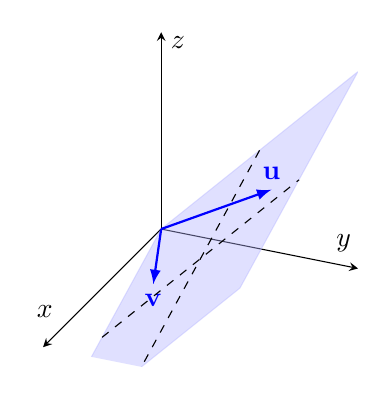
\begin{tikzpicture} 
\begin{axis}[axis lines = center, x={(-0.3cm, -0.3cm)}, y={(.5cm, -0.1cm)}, 
z = {(0cm, 0.5cm)}, xmin = 0, ymin = 0, zmin = 0, xmax = 5, ymax = 5, 
zmax = 5, ticks=none, xlabel = {$x$}, ylabel = {$y$}, zlabel = {$z$}]
    \draw[blue!30, fill = blue!30, opacity = 0.4] (0,0,0) -- (5, 0, -2.5) -- 
    (5, 5, 2.5) -- (0, 5, 5) -- cycle;
    \draw[blue, thick, -latex] (0,0,0) -- (2, 4, 3) node[above] {\textbf{u}};
    \draw[blue, thick, -latex] (0,0,0) -- (2, 1, 0) node[below] {\textbf{v}};
    \draw[black, dashed] (2.5, 0, -1.25) -- (2.5, 5, 3.75);
    \draw[black, dashed] (0, 2.5, 2.5) -- (5, 2.5, 0);
\end{axis}
\end{tikzpicture}
\caption{Linearly independent 3-dimensional vectors, \textbf{u} and \textbf{v}, 
define a plane.}
\label{fig:plane}
\end{figure}

If we have 3 independent vectors, then we can define a \textit{3-dimensional 
space}. To understand this, first imagine a plane formed by two independent 
3-dimensional vectors like in figure \ref{fig:plane}). If a third independent 
vector is introduced, it must not lie on the plane: if it did, it would be a 
linear combination of the first two and therefore not independent. This third 
vector allows us to move off the plane, and therefore all three independent 
vectors span $\mathbb{R}^3$. 

In review, 1 vector or set of dependent vectors 
span a \textit{line}, 2 vectors or sets of dependent vectors span a 
\textit{plane}, and 3 vectors or sets of dependent vectors span $\mathbb{R}^3$. 

\textbf{Example}: Do the vectors $\mathbf{r} = \left[ 5, 4, -6 \right]$, 
$\mathbf{s} = \left[ 0, -5, -10 \right]$, and $\mathbf{t} = \left[ 0, 2, 4, 
\right]$ span a line, plane, or $\mathbb{R}^3$?

\textbf{Solution}: We need to determine the number of \textit{independent 
vectors}. First, we'll check if \textbf{r} and \textbf{s} are independent. 
They are independent if the only solution to the equation below is $a_1 = a_2 
= 0$:
$$a_1 \left[5, 4, -6 \right] + a_2 \left[ 0, -5, -10 \right] = \left[ 0, 0, 0 
\right]$$

Which we can write as a system of equations:
$$5a_1 + 0a_2 = 0$$
$$4a_1 - 5a_2 = 0$$
$$-6a_2 -10a_2 = 0$$

From the first equation, we see that $5a_1 = 0$ which implies that $a_1 = 0$. 
Substituting that into the second equation:
$$4(0) - 5a_2 = 0$$
$$-5a_2 = 0$$
$$a_2 = 0$$

Therefore, vectors \textbf{r} and \textbf{s} are independent. Now let's check 
\textbf{r} and \textbf{t}:
$$a_1 \left[5, 4, -6 \right] + a_2 \left[ 0, 2, 4, \right] = \left[ 0, 0, 0 
\right]$$

Which we can re-write as a system of equations:
$$5a_1 + 0a_2 = 0$$
$$4a_1 + 2a_2 = 0$$
$$-6a_1 + 4a_2 = 0$$

Again, from the first equation, we see that $a_1 = 0$. Substituting into the 
second:
$$4(0) + 2a_2 = 0$$
$$2a_2 = 0$$
$$a_2 = 0$$

Therefore, \textbf{r} and \textbf{t} are also independent. Last, we'll check 
\textbf{s} and \textbf{t} for independence:
$$a_1 \left[0, -5, -10 \right] + a_2 \left[ 0, 1, 2, \right] = \left[ 0, 0, 0 
\right]$$

The system of equations:
$$0a_1 + 0a_2 = 0$$
$$-5a_1 + a_2 = 0$$
$$-10a_1 + 2a_2 = 0$$

The first equation doesn't tell us anything, since it would be true no matter 
what $a_1$ and $a_2$ are. We can solve the second equation for $a_2$ and 
substitute into the third equation:
$$a_2 = 5a_1$$
$$-10a_1 + 2 \left(5a_1 \right) = 0$$
$$-10a_1 + 10a_1 = 0$$

Which is also true for all $a_1$. In fact, there are many solutions to $a_1 
\left[0, -5, -10 \right] + a_2 \left[ 0, 1, 2, \right] = \left[ 0, 0, 0 
\right]$, $a_1 = 1$ and $a_2 = 5$ is an example. Therefore, \textbf{s} and 
\textbf{t} are \textit{dependent}. So, we really have 2 independent vectors in 
the list, and therefore $\text{span}(\mathbf{r}, \mathbf{s}, \mathbf{t})$ is a 
plane. 

\begin{Exercise}[title = {Determining Span}, label = span1]
Geometrically describe (line, plane, or $\mathbb{R}^3$) the span of the list 
of vectors.
\begin{enumerate}
\item $\left[ 1, 2, 4 \right]$ and $\left[-2, -4, -8 \right]$
\item $\left[ 2, 0, 0 \right]$ and $\left[ 0, 1, 3 \right]$
\item $\left[ 3, 0, 0 \right]$ and $\left[ 0, 3, 3 \right]$ and $\left[3, 3, 2 
\right]$
\end{enumerate}
\end{Exercise}

\begin{Answer}[ref = span1]
\begin{enumerate}
\item Since the second vector is a scalar multiple of the first, the span of 
$S = \{ \left[1, 2, 4 \right], \left[-2, -4, -8 \right] \}$ is a \textit{line}.
\item Since the second vector is not a scalar multiple of the first, the span 
of $S = \{ \left[2, 0, 0, \right], \left[0, 1, 3 \right] \}$ is a 
\textit{plane}.
\item None of the three vectors are scalar multiples or linear combinations of 
the other two. Therefore, the span of $S = \{ \left[3, 0, 0 \right], \left[ 0, 
3, 3 \right], \left[3, 3, 2 \right] \}$ is $\mathbb{R}^3$.
\end{enumerate}
\end{Answer}


\section{Determinants}
Checking all these vectors by hand takes a long time. What if you had a list 
of 5, 10, or even 100 vectors? The determinant of a matrix is a scalar value 
that indicates whether the columns of a matrix are linearly independent. So, 
if you put all your vectors together in a matrix and take the determinant of 
that matrix, the result will tell you if all the vectors are independent or 
not. For a 2D matrix, the determinant is the area of the parallelogram defined 
by the column vectors. For a 3D matrix, the determinant is the volume of the 
parallelepiped (a six-dimensional figure formed by six parallelograms, such as 
a cube).\footnote{Note that determinants can only be found for $n \times n$ matrices.} \index{determinant}

Let's plot the parallelogram for this matrix (see figure \ref{fig:twos}):
$$
\begin{bmatrix}
2 & 0  \\
0 & 2 
\end{bmatrix}
$$

\begin{figure}[htbp]
    \centering
    \begin{tikzpicture}
        \begin{axis}[xmin = 0, xmax = 3, ymin = 0, ymax = 3, xlabel = {$x$}, 
        ylabel = {$y$}, axis lines = center, clip = false]
        	\draw[red!30, fill = red!30, opacity = 0.4] (0,0) -- (2, 0) -- (2, 2) 
        	-- (0, 2) -- cycle;
            \draw[red, thick, -latex] (0,0) -- (2, 0) node[above, black, 
            xshift = -1cm] {$\begin{bmatrix}
                2\\
                0
            \end{bmatrix}$};
            \draw[red, thick, -latex] (0,0) -- (0,2) node[right, black, 
            yshift = -1cm] {$\begin{bmatrix}
                0\\
                2
            \end{bmatrix}$};
            \draw[red, dashed] (2, 0) -- (2, 2);
            \draw[red, dashed] (0, 2) -- (2, 2);
            \draw[black, latex-] (1.2, 0) arc(180:90:0.25);
            \draw[black, latex-] (0, 1) arc(-90:0:0.2);
        \end{axis}
    \end{tikzpicture}
    \caption{A parallelogram constructed from vectors $\left[2, 0 \right]$ and 
    $\left[0, 2 \right]$}
    \label{fig:twos}
\end{figure}
 
The formal definition for calculating the determinant of a 2 by 2 matrix is:
$$det(A) = (a\cdot d)-(b\cdot c)$$
where
$$A = 
\begin{bmatrix}
a & b  \\
c & d 
\end{bmatrix}
$$

For the matrix plotted above, the determinant is $(2*2)-(0*0)$. You can also 
see that 4.0 is the area, base (2) times height (2).

You can use the determinant to see what happens to a shape when it goes 
through a linear transformation. Let's scale the 2 by 2 matrix by 4:
$$
\begin{bmatrix}
8 & 0  \\
0 & 8 
\end{bmatrix}
$$
Plot it (see figure \ref{fig:scaled}):

\begin{figure}[htpb]
    \centering
    \begin{tikzpicture}
        \begin{axis}[xmin = 0, xmax = 9, ymin = 0, ymax = 9, xlabel = {$x$}, 
        ylabel = {$y$}, axis lines = center, clip = false]
            \draw[blue!30, fill = blue!30, opacity = 0.4] (2, 0) -- (8, 0) -- 
            (8, 8) -- (0, 8) -- (0, 2) -- (2, 2) -- cycle;
            \draw[blue, thick, -latex] (0,0) -- (8, 0) node[above, black, 
            font = \scriptsize, xshift = -1.25cm] {$\begin{bmatrix}
                8\\
                0
            \end{bmatrix}$};
            \draw[black, latex-] (7.5, 0) arc (0:90:0.75);
            \draw[blue, thick, -latex] (0,0) -- (0,8) node[right, black, 
            font = \scriptsize, yshift = -0.5cm] {$\begin{bmatrix}
                0\\
                8
            \end{bmatrix}$};
            \draw[black, latex-] (0,6) arc (-90:0:0.5);
            \draw[blue, dashed] (8, 0) -- (8, 8);
            \draw[blue, dashed] (8, 8) -- (0,8);
            
            
        \end{axis}
    \end{tikzpicture}
    \caption{Scaling the matrix also scales the parallelogram.}
    \label{fig:scaled}
\end{figure}

Find the determinant. 

$$(8*8)-(0*0) = 64$$

You can see that scaling the matrix scaled the area by the scaling factor 
squared (see figure \ref{fig:both}).

\begin{figure}[htpb]
    \centering
    \begin{tikzpicture}
        \begin{axis}[xmin = 0, xmax = 9, ymin = 0, ymax = 9, xlabel = {$x$}, 
        ylabel = {$y$}, axis lines = center, clip = false]
            \draw[blue!30, fill = blue!30, opacity = 0.4] (2, 0) -- (8, 0) -- 
            (8, 8) -- (0, 8) -- (0, 2) -- (2, 2) -- cycle;
            \draw[blue, thick, -latex] (0,0) -- (8, 0) node[above, black, 
            font = \scriptsize, xshift = -1.25cm] {$\begin{bmatrix}
                8\\
                0
            \end{bmatrix}$};
            \draw[black, latex-] (7.5, 0) arc (0:90:0.75);
            \draw[blue, thick, -latex] (0,0) -- (0,8) node[right, black, 
            font = \scriptsize, yshift = -0.5cm] {$\begin{bmatrix}
                0\\
                8
            \end{bmatrix}$};
            \draw[black, latex-] (0,6) arc (-90:0:0.5);
            \draw[blue, dashed] (8, 0) -- (8, 8);
            \draw[blue, dashed] (8, 8) -- (0,8);
            
            \draw[red!30, fill = red!30, opacity = 0.4] (0,0) -- (2, 0) -- 
            (2, 2) -- (0, 2) -- cycle;
            \draw[red, thick, -latex] (0,0) -- (2, 0) node[above, black, 
            font = \scriptsize, xshift = 0.25cm] {$\begin{bmatrix}
                2\\
                0
            \end{bmatrix}$};
            \draw[black, latex-] (1.2, 0) arc(180:90:0.75);
            \draw[red, thick, -latex] (0,0) -- (0,2) node[right, black, 
            font = \scriptsize, yshift = 0.4cm] {$\begin{bmatrix}
                0\\
                2
            \end{bmatrix}$};
            \draw[black, latex-] (0, 1.5) arc(-90:0:0.5);
            \draw[red, dashed] (2, 0) -- (2, 2);
            \draw[red, dashed] (0, 2) -- (2, 2);
            
            
        \end{axis}
    \end{tikzpicture}
    \caption{Scaling a matrix by a constant $c$ increases the area of the 
    parallelogram by a factor of $c^2$.}
    \label{fig:both}
\end{figure}

We can show why this is true mathematically. Suppose we have a 2 by 2 matrix A:
$$A = \begin{bmatrix}
w & x\\
y & z
\end{bmatrix}$$

Then $det(A) = wz - xy$. We can scale this matrix by a constant, $c$:
$$cA = c \cdot \begin{bmatrix}
w & x\\
y & z
\end{bmatrix} = \begin{bmatrix}
cw & cx\\
cy & cz
\end{bmatrix}$$

And we can take the determinant:
$$det(cA) = det \left( \begin{bmatrix}
cw & cx\\
cy & cz
\end{bmatrix} \right)= cw(cz) - cx(cy) = c^2 (wz - xy) = c^2 \cdot det(A)$$

Therefore, scaling a 2 by 2 matrix by a factor changes the determinant by that 
factor squared. What about higher dimensions? If each side of a cube were 
scaled by a factor of $c$, then the volume of the cube would change by a 
factor of $c^3$ (feel free to confirm this yourself). And if a tesseract (a 
four-dimensional cube) had each side scaled by a factor of $c$, then the 
hypervolume (four-dimensional volume) would be scaled by a factor of $c^4$. Do 
you notice a pattern?

In fact, scaling an $n \times n$ matrix by a constant factor, $c$, changes the 
determinant of that $n \times n$ matrix by a factor of $c^n$. 

What happens if the columns of a matrix are not independent? Let's plot this 
matrix (see figure \ref{fig:zero_det}):
$$
\begin{bmatrix}
2 & 1  \\
4 & 2 
\end{bmatrix}
$$

\begin{figure}[htbp]
    \centering
    \begin{tikzpicture}
        \begin{axis}[xmin = 0, ymin = 0, xmax = 4, ymax = 5, xlabel = {$x$}, 
        ylabel = {$y$}, axis lines = center]
            \draw[red, thick, -latex] (0,0) -- (2, 4) node[below, black, 
            font = \scriptsize, yshift = -0.5cm] {$\begin{bmatrix}
                2\\
                4
            \end{bmatrix}$};
            \draw[-latex] (2, 2.9) arc (0:-120:0.5);
            \draw[blue, thick, -latex] (0,0) -- (1, 2) node[above, black, 
            font = \scriptsize, xshift = -0.75cm, yshift = -0.75cm] {$\begin{bmatrix}
                1\\
                2
            \end{bmatrix}$};
            \draw[-latex] (0.4, 1.6) arc (90:280:0.3);
        \end{axis}
    \end{tikzpicture}
    \caption{The vectors $\begin{bmatrix} 1\\2 \end{bmatrix}$ and 
    $\begin{bmatrix} 2\\4 \end{bmatrix}$ are co-linear, so there is no area 
    between them and the determinant of $\begin{bmatrix} 2 & 1\\ 4 & 2 
    \end{bmatrix}$ is zero.}
    \label{fig:zero_det}
\end{figure}

One vector overwrites the other. As you can see, the area is 0 because there 
is no space between the vectors. Therefore, the columns of the matrix are 
linearly dependent.

\begin{Exercise}[title = {Finding the Determinate}, label = geo_det]
Plot the parallelogram represented by the columns of the matrix. What is the 
area of this parallelogram?
\begin{enumerate}
\item $\begin{bmatrix}
1 &4\\
-3 & 1
\end{bmatrix}$
\item $\begin{bmatrix}
5 & -5 \\
5 & -1
\end{bmatrix}$
\item $\begin{bmatrix}
0 & -5 \\
-2 & 0 
\end{bmatrix}$
\end{enumerate}
\end{Exercise}

\begin{Answer}[ref = geo_det]
\begin{enumerate}
    \item Our two vectors from the columns of the matrix are $\left[1, -3 
    \right]$ and $\left[4, 1 \right]$. Plotting:
    
    \begin{tikzpicture}
        \begin{axis}[xmin = -1, xmax = 5, ymin = -4, ymax = 2, xlabel = {$x$}, 
        ylabel = {$y$}, axis lines = center]
            \draw[blue, thick, -latex] (0,0) -- (1, -3);
            \draw[blue, thick, -latex] (0,0) -- (4, 1);
            \draw[blue, dashed] (1, -3) -- (5, -2);
            \draw[blue, dashed] (5, -2) -- (4, 1);
        \end{axis}
    \end{tikzpicture}

    The area of this parallelogram is the same as the determinant of the matrix:
    $$det\left( \begin{bmatrix}
        1 & 4\\
        -3 &1
    \end{bmatrix} \right) = 1 \cdot 1 - \left( 4 \cdot -3 \right) = 1 + 12 = 13$$

    \item Our two vectors from the columns of the matrix are $\left[5, 5 
    \right]$ and $\left[-5, -1 \right]$. Plotting:

    \begin{tikzpicture}
        \begin{axis}[xmin = -6, xmax = 6, ymin = -2, ymax = 6, xlabel = {$x$}, 
        ylabel = {$y$}, axis lines = center]
            \draw[blue, thick, -latex] (0,0) -- (5, 5);
            \draw[blue, thick, -latex] (0,0) -- (-5, -1);
            \draw[blue, dashed] (-5, -1) -- (0, 4);
            \draw[blue, dashed] (0, 4) -- (5, 5);
        \end{axis}
    \end{tikzpicture}

    The area of this parallelogram is the same as the determinant of the 
    matrix:
    $$det \left( \begin{bmatrix}
        5 & -5\\
        5 & -1
    \end{bmatrix} \right) = 5 \cdot -1 - \left( -5 \cdot 5 \right) = -5 + 25 = 
    20$$

    \item Our two vectors from the columns of the matrix are $\left[ 0, -2 
    \right]$ and $\left[ -5, 0 \right]$. Plotting:

    \begin{tikzpicture}
        \begin{axis}[xmin = -6, xmax = 1, ymin = -2, ymax = 1, xlabel = {$x$}, 
        ylabel = {$y$}, axis lines = center]
            \draw[blue, thick, -latex] (0,0) -- (0, -2);
            \draw[blue, thick, -latex] (0,0) -- (-5, 0);
            \draw[blue, dashed] (-5, 0) -- (-5, -2);
            \draw[blue, dashed] (-5, -2) -- (0, -2);
        \end{axis}
    \end{tikzpicture}

    This is a rectangle, and we can see the area is $5 \cdot 2 = 10$. However, 
    the determinant is:
    $$det \left( \begin{bmatrix}
        0 & -5\\
        -2 & 0
    \end{bmatrix} \right) = 0 \cdot 0 - \left( -5 \cdot -2 \right) = 0 - 10 = 
    -10$$

    We will discuss this unusual response in a future chapter. 
\end{enumerate}
\end{Answer}

Calculating the determinant for a 2 by 2 matrix is easy. For a larger matrix, 
finding the determinant is more complex and requires breaking down the matrix 
into smaller matrices until you reach the 2x2 form. The process is called 
expansion by minors. For our purposes, we simply want to first check to see if 
a matrix contains linearly independent rows and columns before using our 
Python code to solve. 

Modify your code so that is uses the $np.linalg.det()$ function. If the 
determinant is not zero, then you can call the $np.linalg.solve()$ function. 
Your code should look like this:
\begin{Verbatim}
if (np.linalg.det(D) != 0):
    j = np.linalg.solve(D,e)
    print(j)
else:
     print("Rows and columns are not independent.")
\end{Verbatim}

\section{Where to Learn More}
Watch this video on \emph {Linear Combinations and Vector Spans from Khan 
Academy}: \url{http://rb.gy/g1snk}

The Wolfram Demonstrations website has a fun, interactive demo where you can 
enter values for 2D and 3D matrices and see how the area or volume changes. 
\url{https://demonstrations.wolfram.com/DeterminantsSeenGeometrically/#more}

If you are curious about the \emph {Expansion of Minors}, see:
\url {https://mathworld.wolfram.com/DeterminantExpansionbyMinors.html}